%20/03 - Carlos Aguirre
\chapter{Teoría de grafos y métricas}
\section{Introducción a la teoría de grafos}
La teoría de grafos ha sido utilizada recientemente para:
\begin{itemize}
\item Clasificación automática de secuencias de proteínas.
\item Detección de jerarquías de proteínas.
\item Análisis de redes genéticas.
\item Reconstrucción de redes genéticas grandes obtenidas mediante modificación de genes.
\end{itemize}

Un grafo G es un par de conjuntos (V,E) donde $V = \{v_1, v_2, \ldots v_n\}$ es el conjunto de vértices o nodos y $E = \{(v_i, v_j), (v_{i'}, v_{j'}), \ldots \}$ es un conjunto de pares no ordenados de elementos de V y se denomina conjunto de ramas del grafo. 
\marginpar[\footnotesize Pregunta de test: define orden y tamaño, dado un grafo dar el orden y tamaño, etc. ]  \
El número de nodos se denomina \textbf{orden} del grafo, y el número de ramas es el \textbf{tamaño} del grafo. 

\begin{figure}[h]
\centering
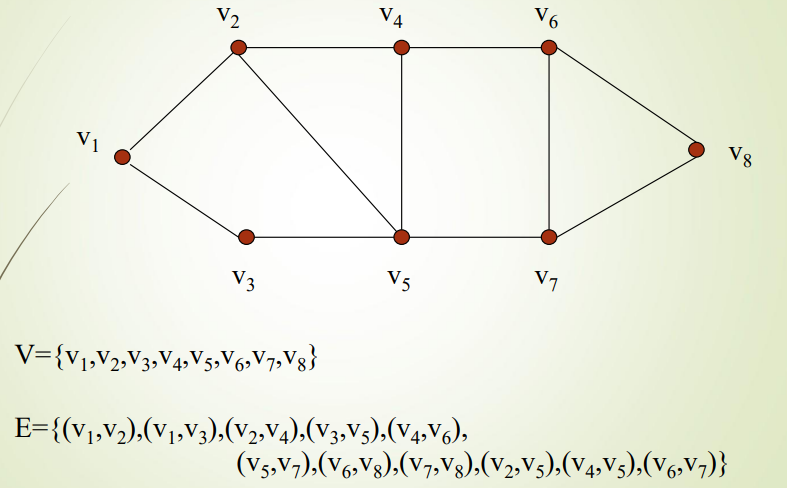
\includegraphics[width = 0.6\textwidth]{figs/grafo.png}
\caption{Ejemplo de grafo de orden 8 y tamaño 11.}
\end{figure}

Para una red de proteínas, cada proteína sería un nodo del grafo, y una rama indicaría interacción entre ambas proteínas. 

Una disposición (layout) es una posible colocación de los nodos y las ramas en un espacio 2D o 3D. Un mismo gráfo puede tener múltiples colocaciones. Ejemplo, consideremos el grafo G=(V,E).

\begin{figure}[h]
\centering
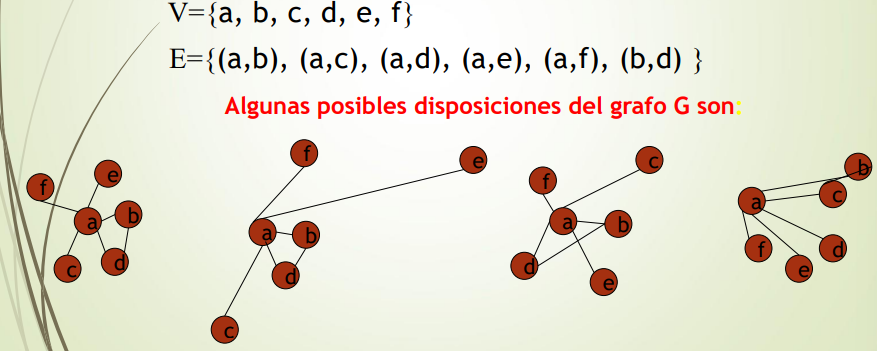
\includegraphics[width = 0.6\textwidth]{figs/layout.png}
\end{figure}

Existen programas de ordenador que nos permiten obtener colocaciones predefinidas (Gephy, Pajek). Cuando no se especifica ninguna colocación, se entiende que los nodos se sitúan aleatoriamente sobre el plano o espacio. Algunos de los tipos más habituales de colocaciones son:
\begin{itemize}
\item Colocaciones regulares
\item Basadas en la física (atracción-repulsión)
\item Basadas en propiedades topológicas (jerarquías, número de vecinos, etc)
\end{itemize}

Un hipergrafo H es un también par de conjuntos (V,E) donde $V=\{v_1, v_2, \ldots v_n\}$ es el conjunto de vértices o nodos y $E=\{(v_{i1}, v_{i2}, \ldots),(v_{i'1},v_{i'2}, \ldots), \ldots\}$ es una familia de
subconjuntos no ordenados de elementos de V. E se denomina conjunto de hiperramas o hiperaristas del hipergrafo. El número de hiperramas $|E|$ se denomina cardinalidad del hipergrafo. El valor $|E|*|V|$ se denomina tamaño o volumen del grafo.
\marginpar[\footnotesize Pregunta examen ]  \
Si tenemos un grafo de n nodos, ¿cuántas parejas podemos tener como máximo? $(n \cdot n-1)/2$ Por tanto, en un grafo con n nodos, ¿cuántas ramas puede tener? Igual, $(n \cdot n-1)/2$

\begin{figure}[h]
\centering
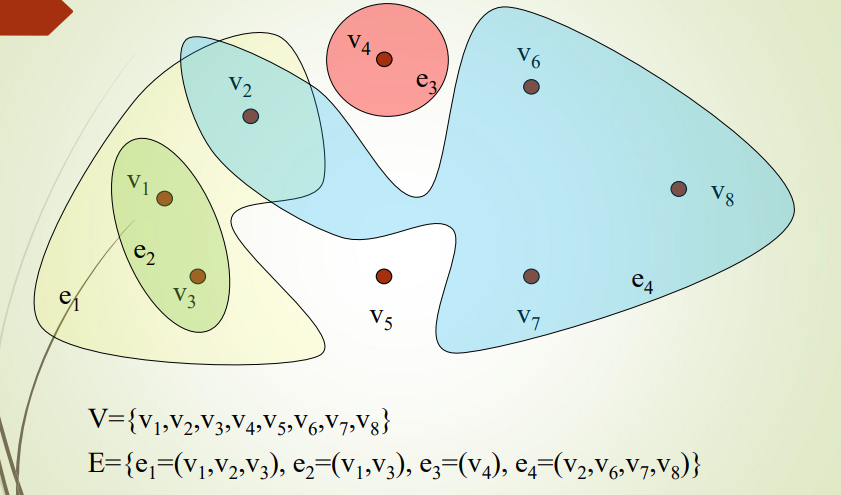
\includegraphics[width = 0.6\textwidth]{figs/hipergrafo.png}
\caption{Ejemplo de hipergrafo de cardinalidad 4 y tamaño 32.}
\end{figure}

Un hipergrafo H se dice que es \textbf{propio} si no es vacío ($V\neq \varnothing$) y no contiene ninguna arista vacía. Un hipergrafo H se dice que tiene \textbf{dominio completo} si todos los nodos están en al menos una arista, en caso contrario se dice que tiene \textbf{dominio parcial}. Si en un hipergrafo todas las hiperramas tienen el mismo número de nodos, entonces se denomina \textbf{hipergrafo k-uniforme}. 

\textit{Ejercicio: Indicar si el hipergrafo del ejemplo anterior es propio, tiene dominio completo y si es k uniforme}. Es propio (el conjunto de vértices tiene 8 elementos y todas las ramas e tienen vértices dentro), es de dominio parcial (v5 no está en ninguna rama) y no es k-uniforme (e1 tiene 3 elementos, e2 tiene 2, e3 tiene 1 y e4 tiene 4).

\section{Bucles y ramas paralelas}
Un bucle es una rama que empieza y termina en el mismo nodo $(v_i, v_i)$. Cuando dos ramas conectan el mismo par de vértices se denominan paralelas. Un grafo con bucles se denomina pseudografo. Un grafo con ramas paralelas pero sin bucles se denomina multigrafos. Un grafo sin bucles ni ramas paralelas se denomina grafo simple.

\begin{figure}[h]
\centering
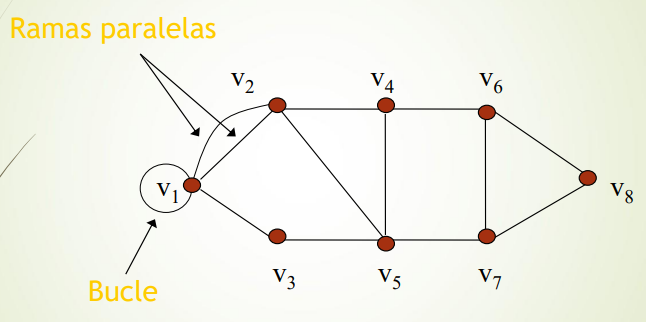
\includegraphics[width = 0.6\textwidth]{figs/bucle-rama-paralela.png}
\end{figure}

\section{Grafos dirigidos y ponderados}
Se puede considerar que los enlaces entre nodos son dirigidos $(v_i, v_j) = (v_j, v_i)$. Los grafos dirigidos se denominan también \textbf{digrafos}.

\begin{figure}[h]
\centering
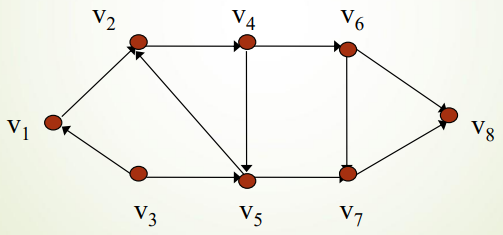
\includegraphics[width = 0.6\textwidth]{figs/grafo-dirigido.png}
\end{figure}

En los grafos ponderados, a cada rama del grafo se le puede asociar un número. El número asociado a cada rama puede indicar entre otras cosas una distancia, una capacidad, un valor temporal, etc.

\begin{figure}[h]
\centering
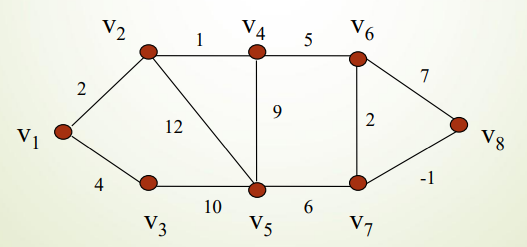
\includegraphics[width = 0.6\textwidth]{figs/grafo-ponderado.png}
\end{figure}

\newpage

Los grafos dirigidos y ponderados poseen ramas dirigidas a las que se asocia un número.

\begin{figure}[h]
\centering
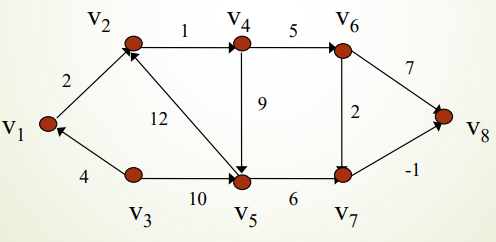
\includegraphics[width = 0.6\textwidth]{figs/grafo-dirigido-ponderado.png}
\end{figure}